\documentclass[/home/jesse/Analysis/FemtoAnalysis/AnalysisNotes/AnalysisNoteJBuxton.tex]{subfiles}
\begin{document}

\subsubsection{\texorpdfstring{$\bar{\Lambda}$K$^{+}$}{TEXT} Residuals}
\label{Residuals_ALamKchP}

\begin{figure}[h]
  \centering
  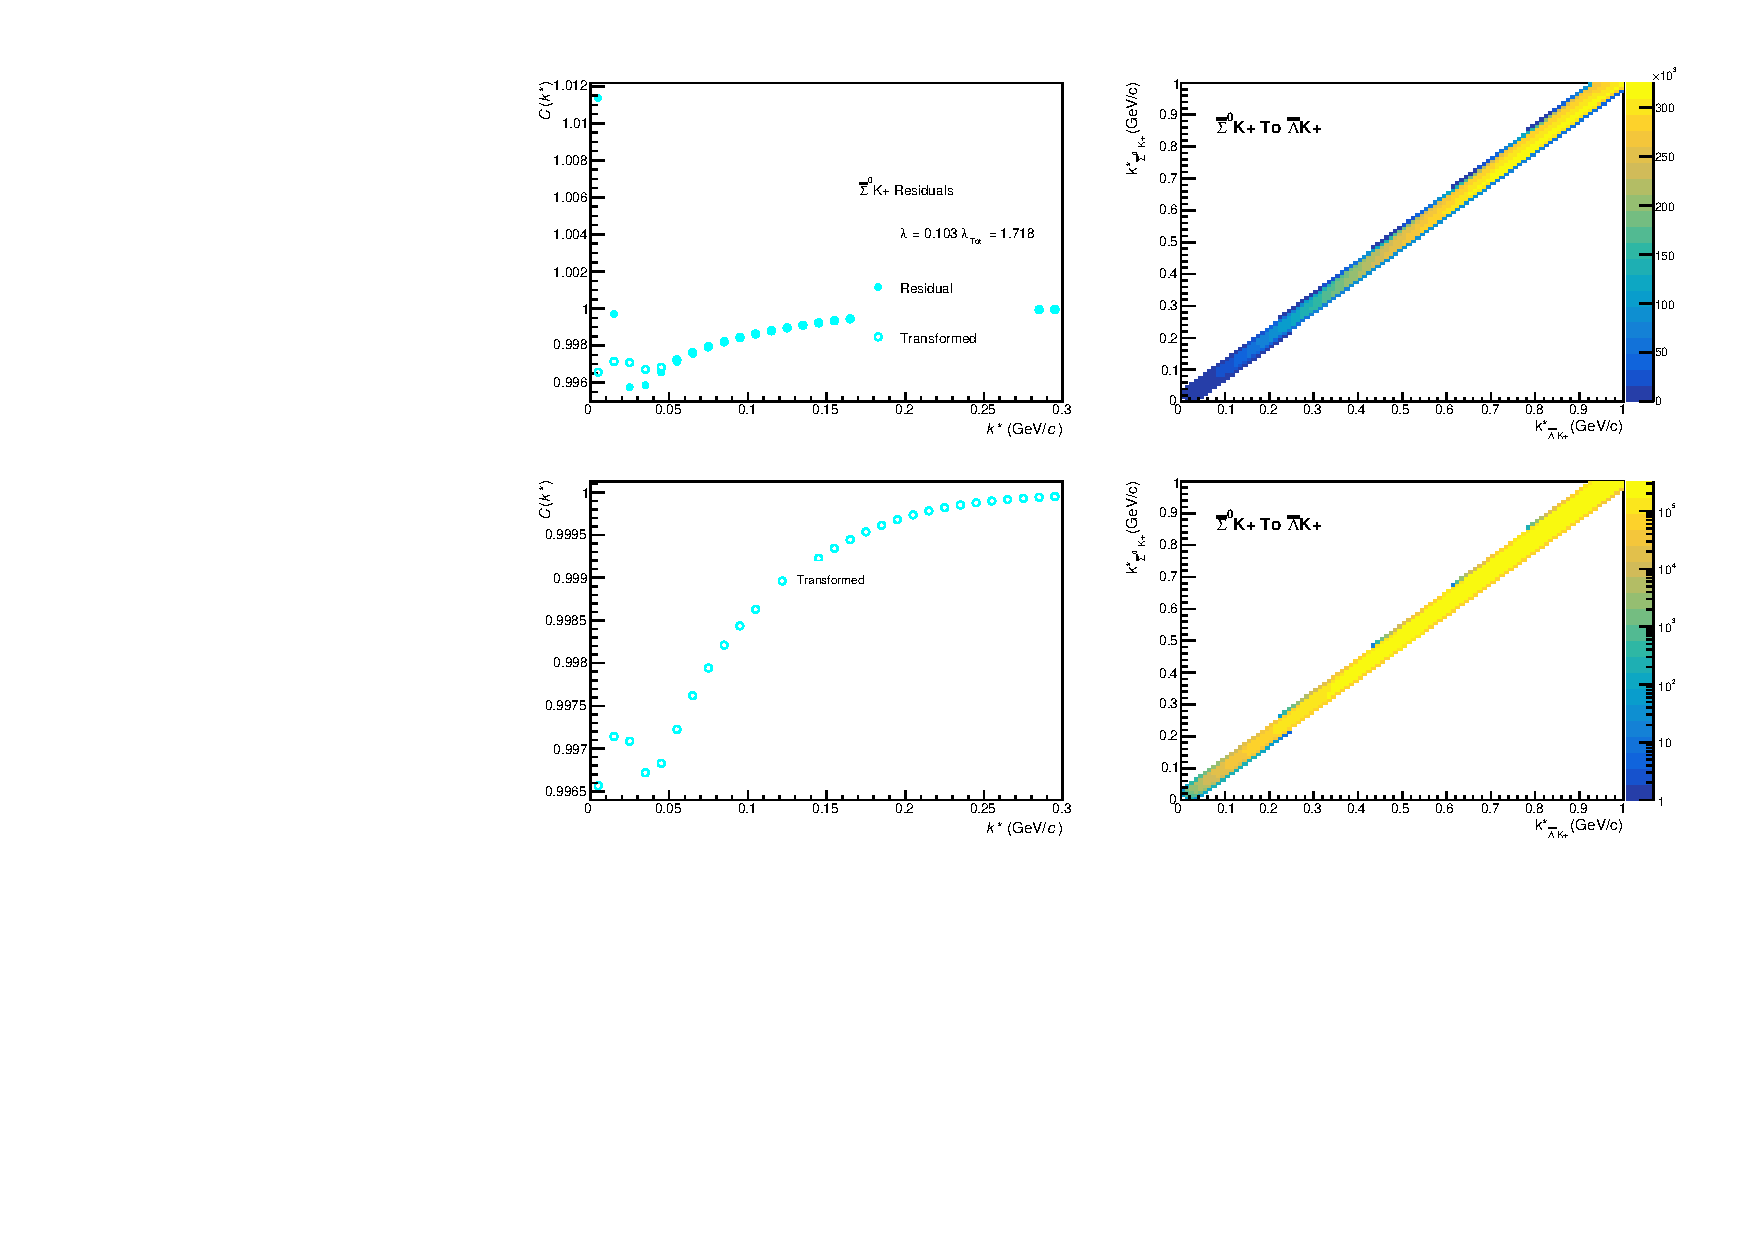
\includegraphics[width=\textwidth]{/home/jesse/Analysis/FemtoAnalysis/AnalysisNotes/Appendices/Appendix_AdditionalFigures/Figures/Residuals/ALamKchP/Residuals_ALamKchP_0010_ASig0KchP_MomResCrctn_NonFlatBgdCrctn_10Res_PrimMaxDecay4fm_UsingXiDataAndCoulombOnly.pdf}
  \caption[Residuals: $\bar{\Sigma}^{0}$K$^{+}$ to $\bar{\Lambda}$K$^{+}$ (0-10\% Centrality)]{Residuals: $\bar{\Sigma}^{0}$K$^{+}$ to $\bar{\Lambda}$K$^{+}$ (0-10\% Centrality)}
  \label{fig:Res_ALamKchP_0010_ASig0KchP}
\end{figure}

\begin{figure}[h]
  \centering
  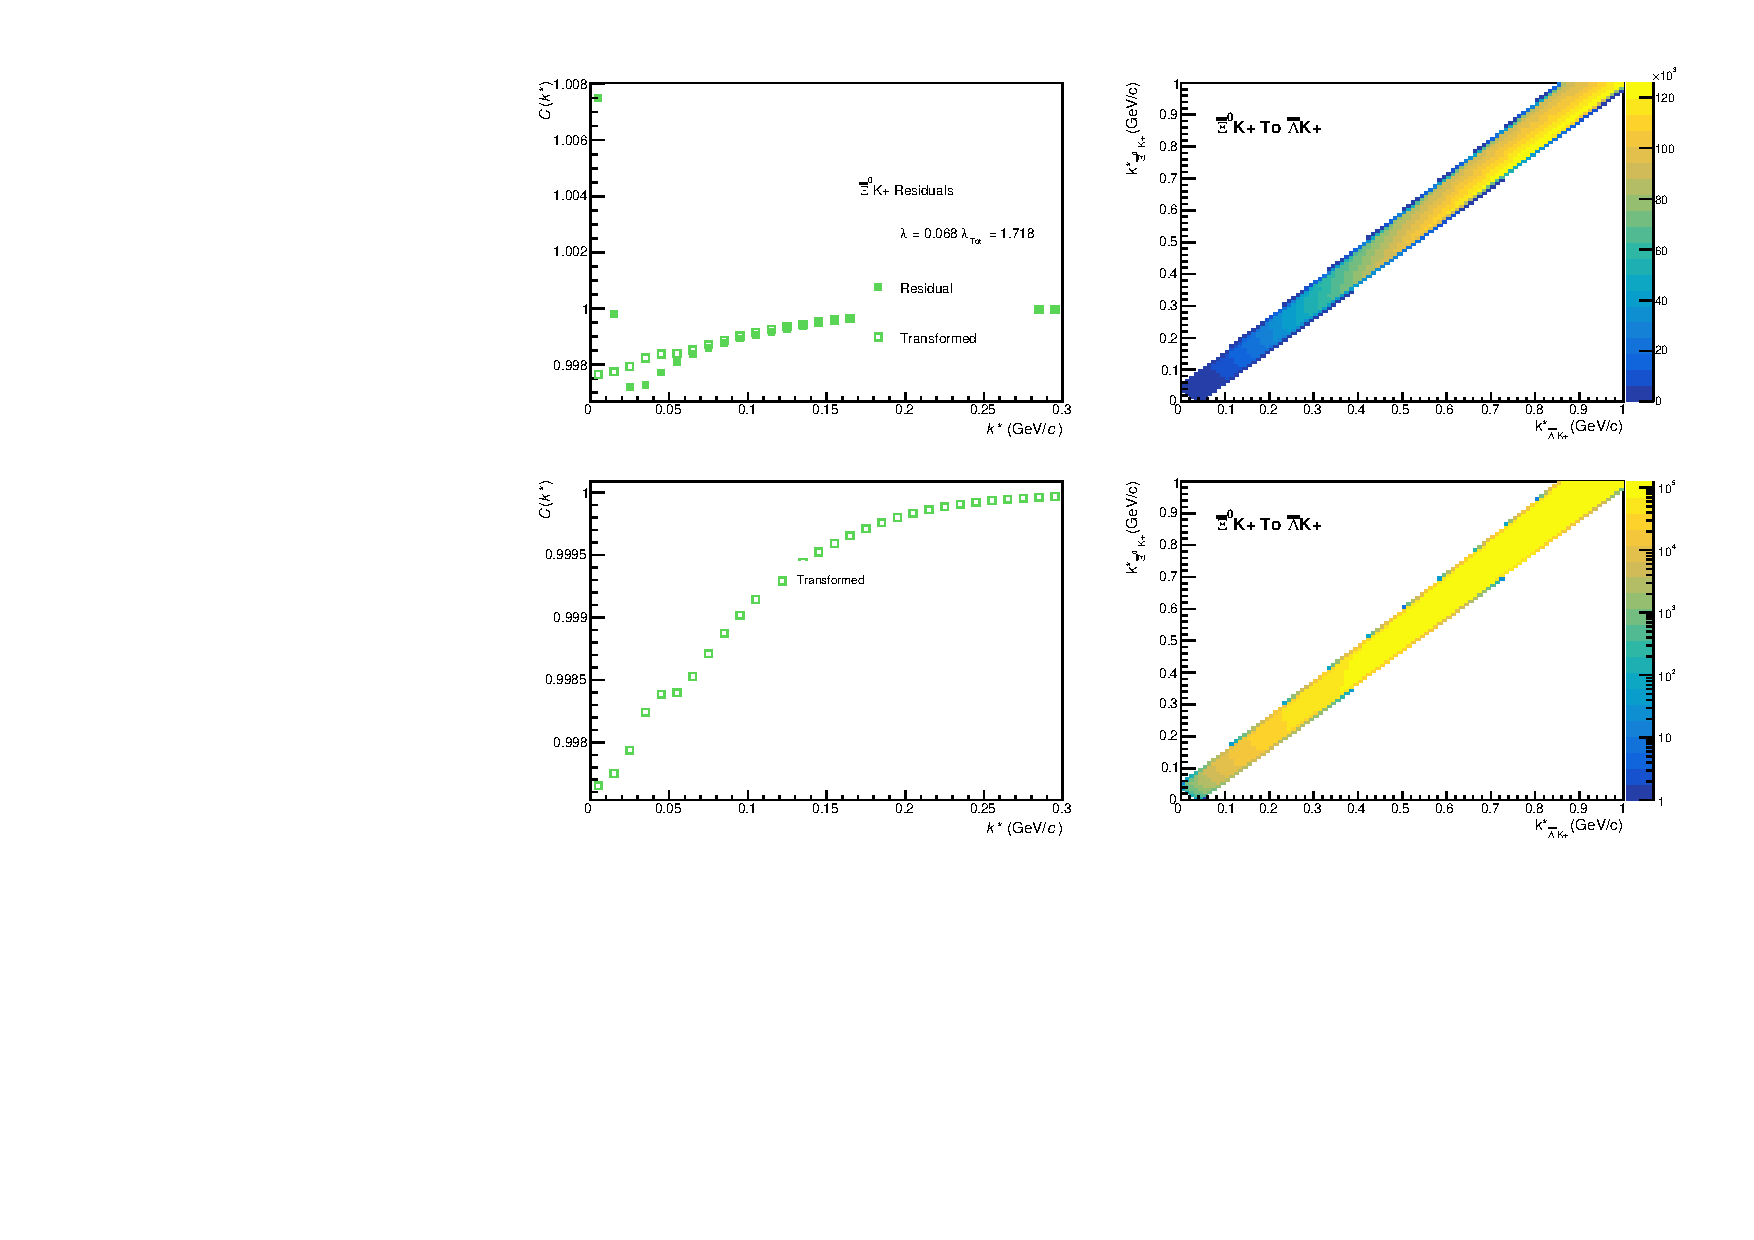
\includegraphics[width=\textwidth]{/home/jesse/Analysis/FemtoAnalysis/AnalysisNotes/Appendices/Appendix_AdditionalFigures/Figures/Residuals/ALamKchP/Residuals_ALamKchP_0010_AXi0KchP_MomResCrctn_NonFlatBgdCrctn_10Res_PrimMaxDecay4fm_UsingXiDataAndCoulombOnly.pdf}
  \caption[Residuals: $\bar{\Xi}^{0}$K$^{+}$ to $\bar{\Lambda}$K$^{+}$ (0-10\% Centrality)]{Residuals: $\bar{\Xi}^{0}$K$^{+}$ to $\bar{\Lambda}$K$^{+}$ (0-10\% Centrality)}
  \label{fig:Res_ALamKchP_0010_AXi0KchP}
\end{figure}


\begin{figure}[h]
  \centering
  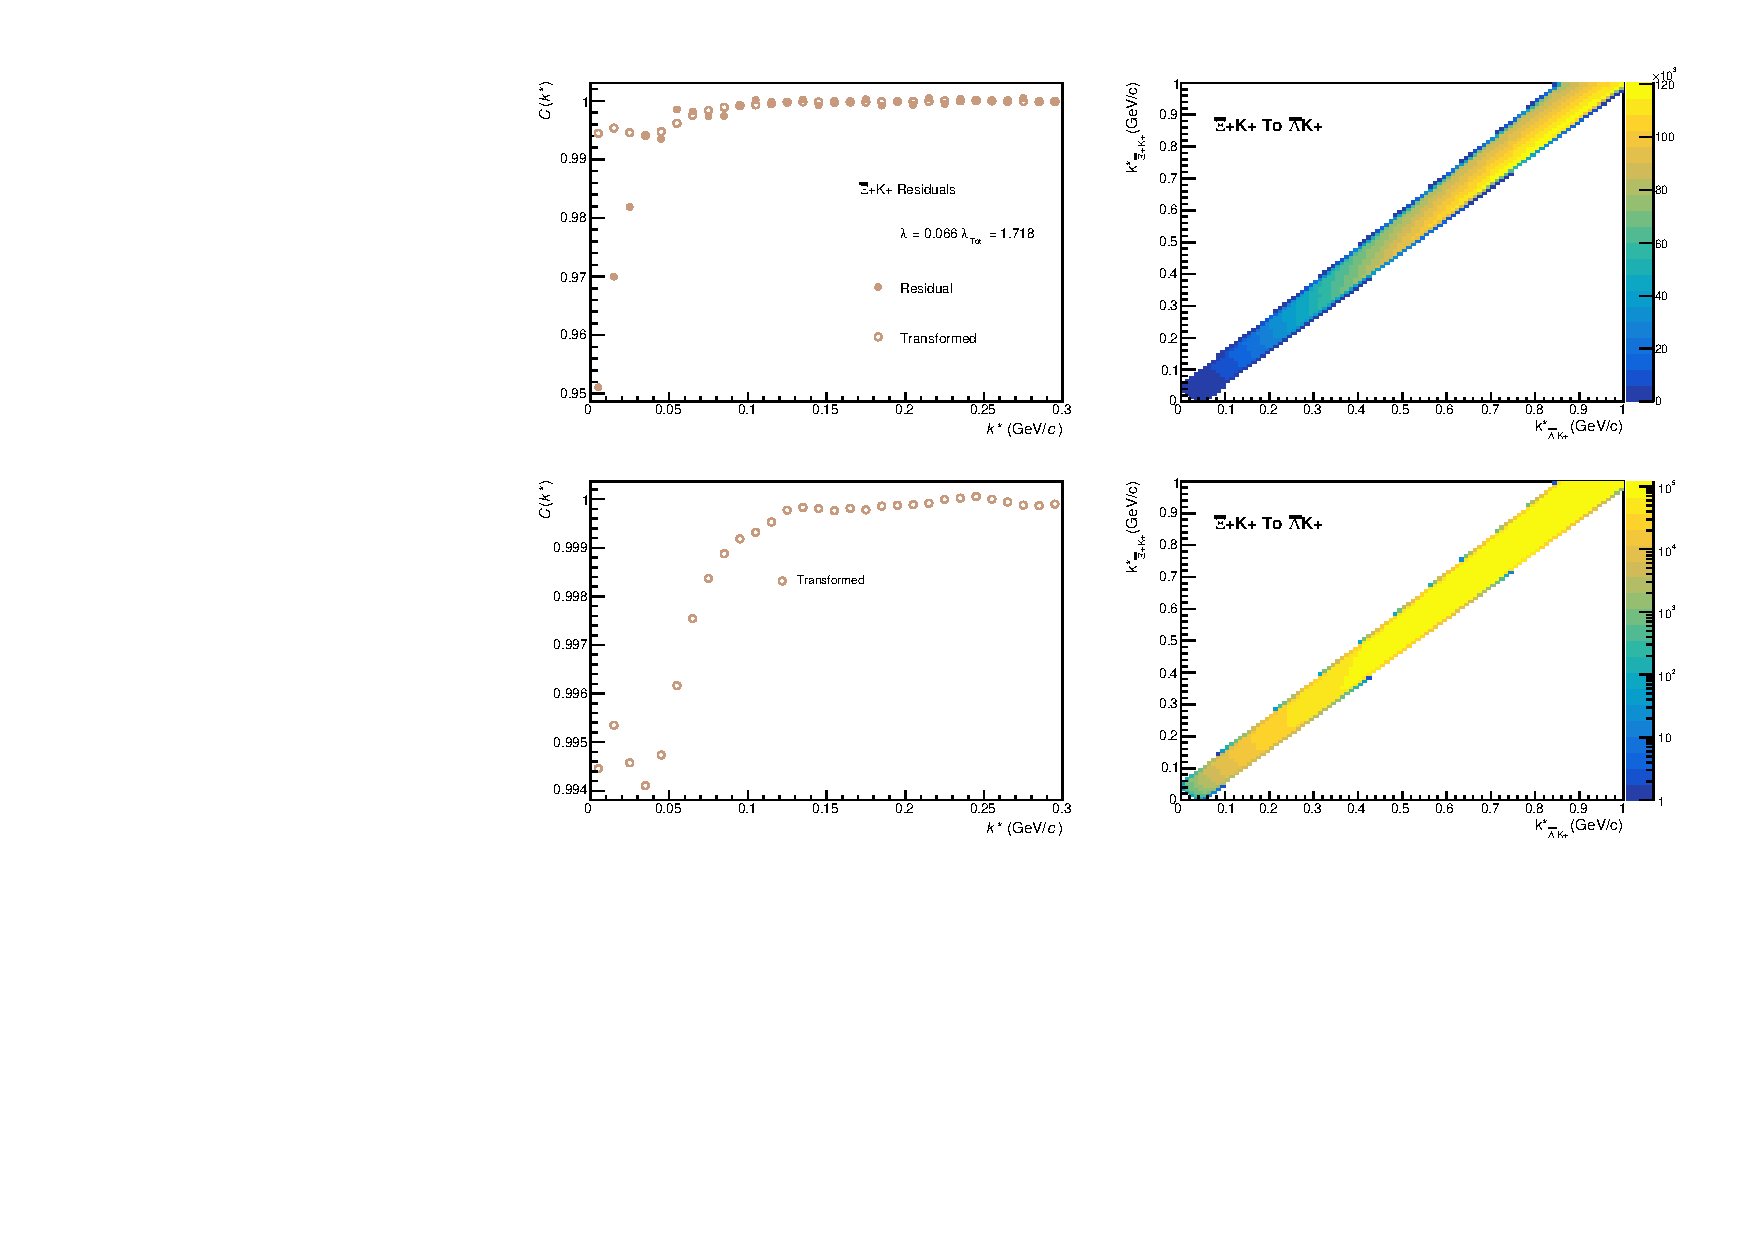
\includegraphics[width=\textwidth]{/home/jesse/Analysis/FemtoAnalysis/AnalysisNotes/Appendices/Appendix_AdditionalFigures/Figures/Residuals/ALamKchP/Residuals_ALamKchP_0010_AXiKchP_MomResCrctn_NonFlatBgdCrctn_10Res_PrimMaxDecay4fm_UsingXiDataAndCoulombOnly.pdf}
  \caption[Residuals: $\bar{\Xi}^{+}$K$^{+}$ to $\bar{\Lambda}$K$^{+}$ (0-10\% Centrality)]{Residuals: $\bar{\Xi}^{+}$K$^{+}$ to $\bar{\Lambda}$K$^{+}$ (0-10\% Centrality)}
  \label{fig:Res_ALamKchP_0010_AXiCKchP}
\end{figure}


\begin{figure}[h]
  \centering
  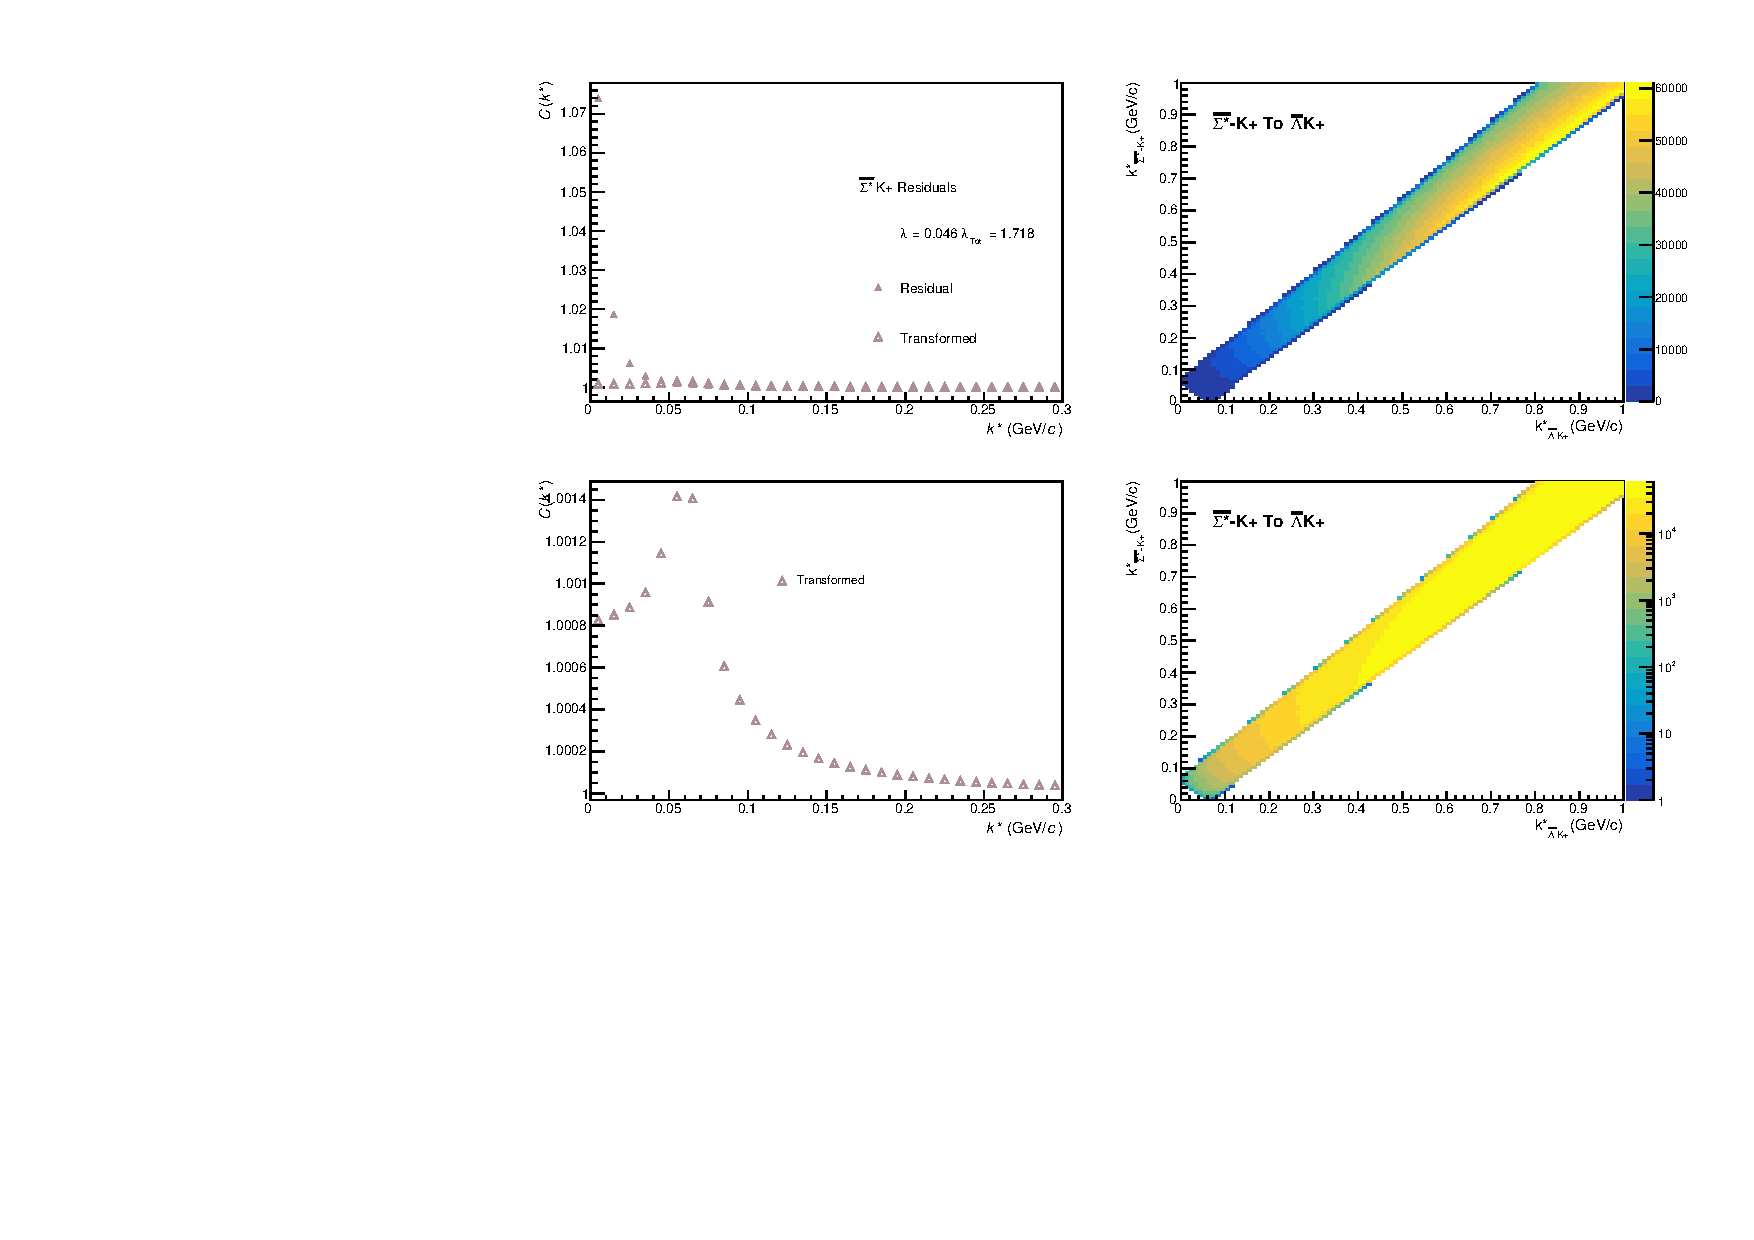
\includegraphics[width=\textwidth]{/home/jesse/Analysis/FemtoAnalysis/AnalysisNotes/Appendices/Appendix_AdditionalFigures/Figures/Residuals/ALamKchP/Residuals_ALamKchP_0010_ASigStMKchP_MomResCrctn_NonFlatBgdCrctn_10Res_PrimMaxDecay4fm_UsingXiDataAndCoulombOnly.pdf}
  \caption[Residuals: $\bar{\Sigma}^{*-}$K$^{+}$ to $\bar{\Lambda}$K$^{+}$ (0-10\% Centrality)]{Residuals: $\bar{\Sigma}^{*-}$K$^{+}$ to $\bar{\Lambda}$K$^{+}$ (0-10\% Centrality)}
  \label{fig:Res_ALamKchP_0010_ASigStMKchP}
\end{figure}

\begin{figure}[h]
  \centering
  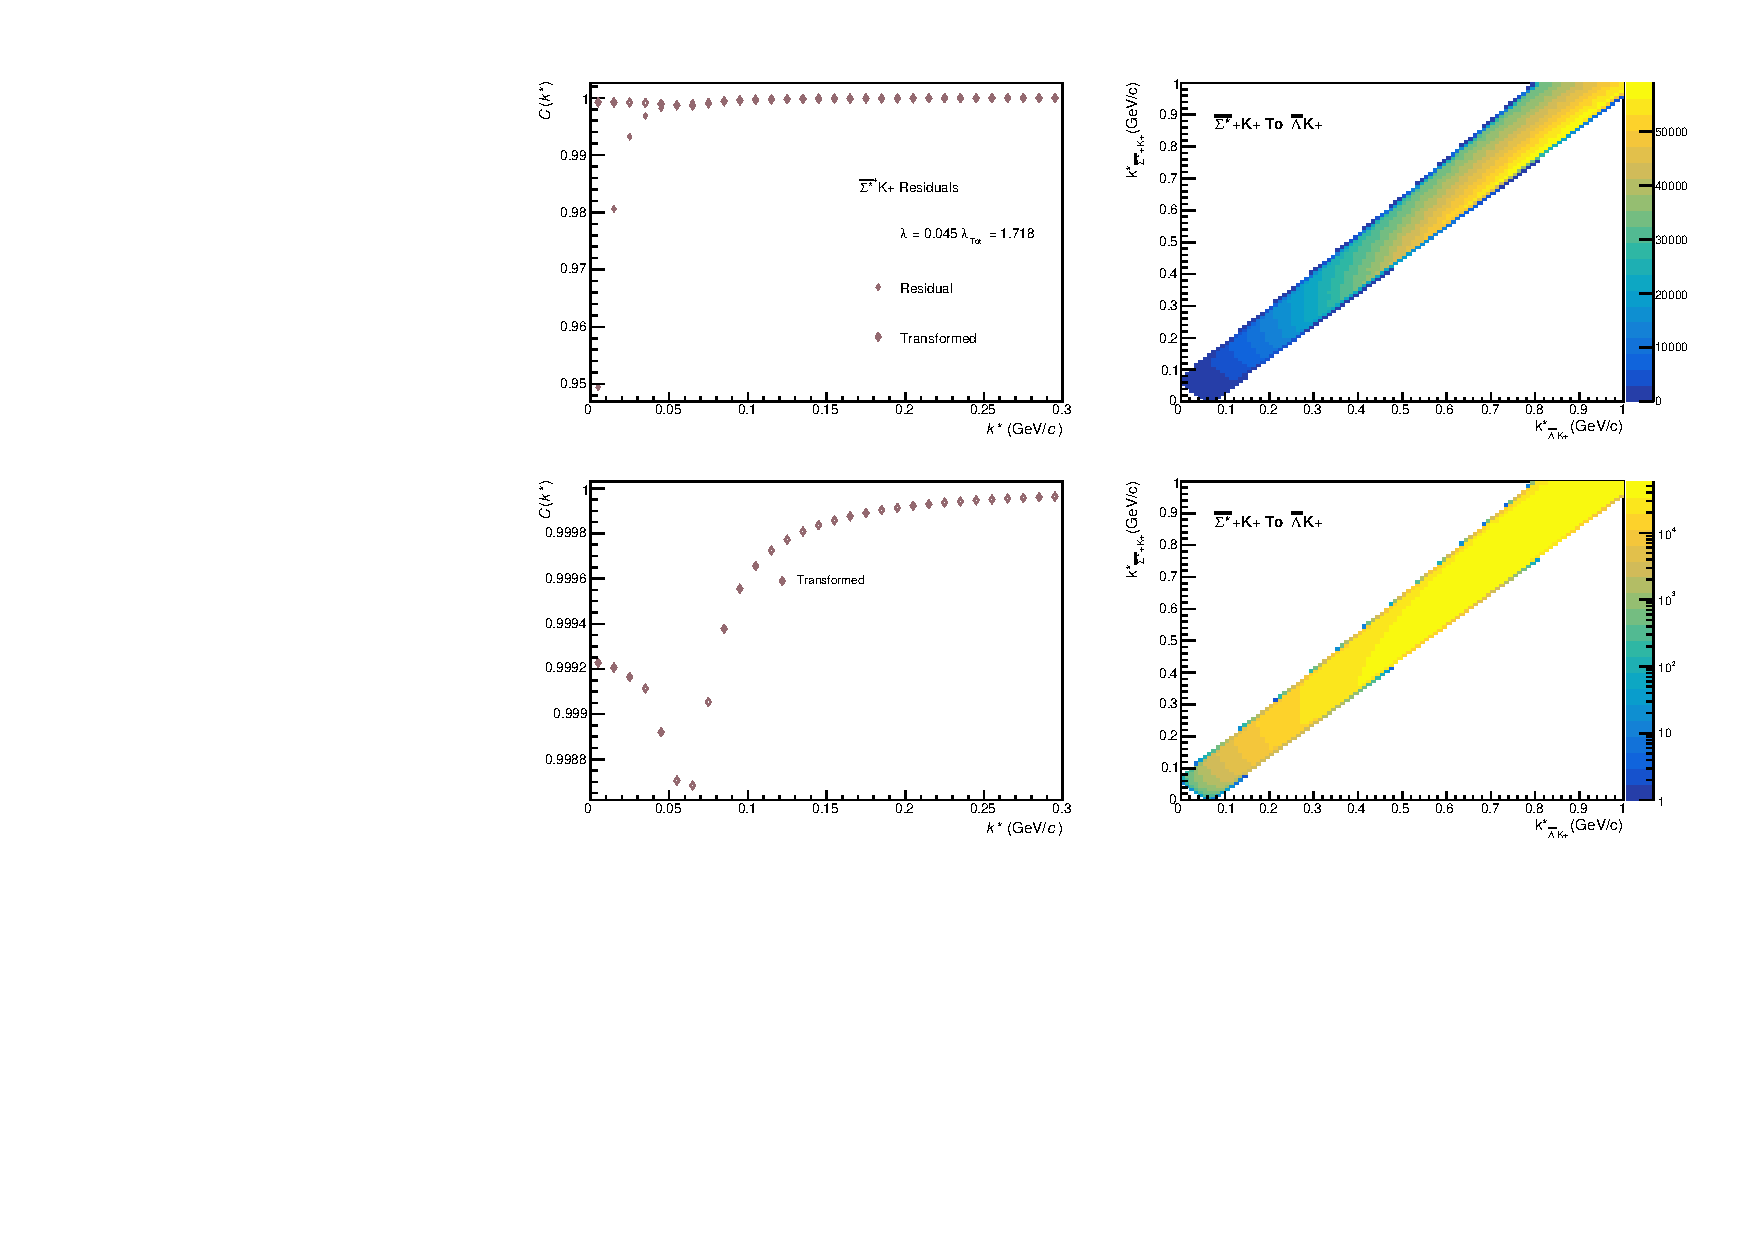
\includegraphics[width=\textwidth]{/home/jesse/Analysis/FemtoAnalysis/AnalysisNotes/Appendices/Appendix_AdditionalFigures/Figures/Residuals/ALamKchP/Residuals_ALamKchP_0010_ASigStPKchP_MomResCrctn_NonFlatBgdCrctn_10Res_PrimMaxDecay4fm_UsingXiDataAndCoulombOnly.pdf}
  \caption[Residuals: $\bar{\Sigma}^{*+}$K$^{+}$ to $\bar{\Lambda}$K$^{+}$ (0-10\% Centrality)]{Residuals: $\bar{\Sigma}^{*+}$K$^{+}$ to $\bar{\Lambda}$K$^{+}$ (0-10\% Centrality)}
  \label{fig:Res_ALamKchP_0010_ASigStPKchP}
\end{figure}

\begin{figure}[h]
  \centering
  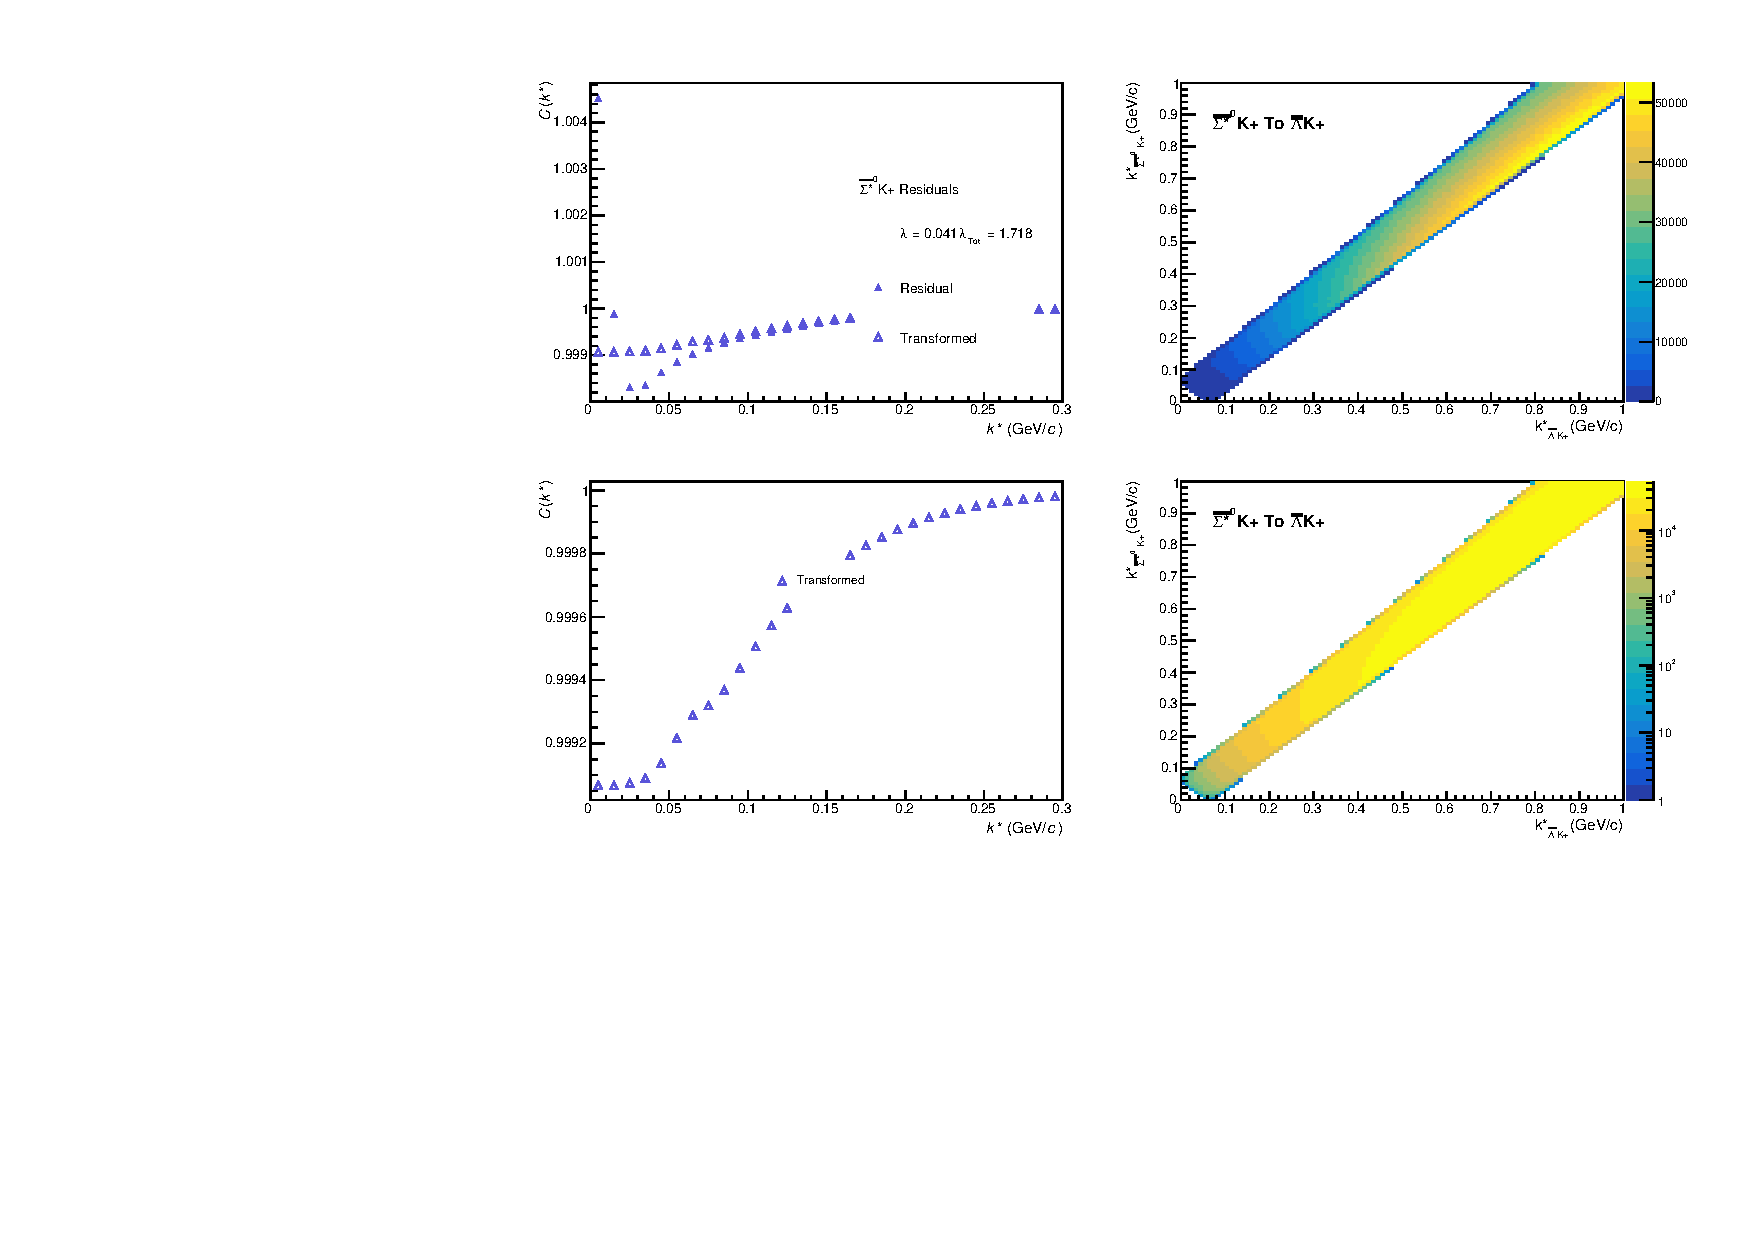
\includegraphics[width=\textwidth]{/home/jesse/Analysis/FemtoAnalysis/AnalysisNotes/Appendices/Appendix_AdditionalFigures/Figures/Residuals/ALamKchP/Residuals_ALamKchP_0010_ASigSt0KchP_MomResCrctn_NonFlatBgdCrctn_10Res_PrimMaxDecay4fm_UsingXiDataAndCoulombOnly.pdf}
  \caption[Residuals: $\bar{\Sigma}^{*0}$K$^{+}$ to $\bar{\Lambda}$K$^{+}$ (0-10\% Centrality)]{Residuals: $\bar{\Sigma}^{*0}$K$^{+}$ to $\bar{\Lambda}$K$^{+}$ (0-10\% Centrality)}
  \label{fig:Res_ALamKchP_0010_ASigSt0KchP}
\end{figure}


\begin{figure}[h]
  \centering
  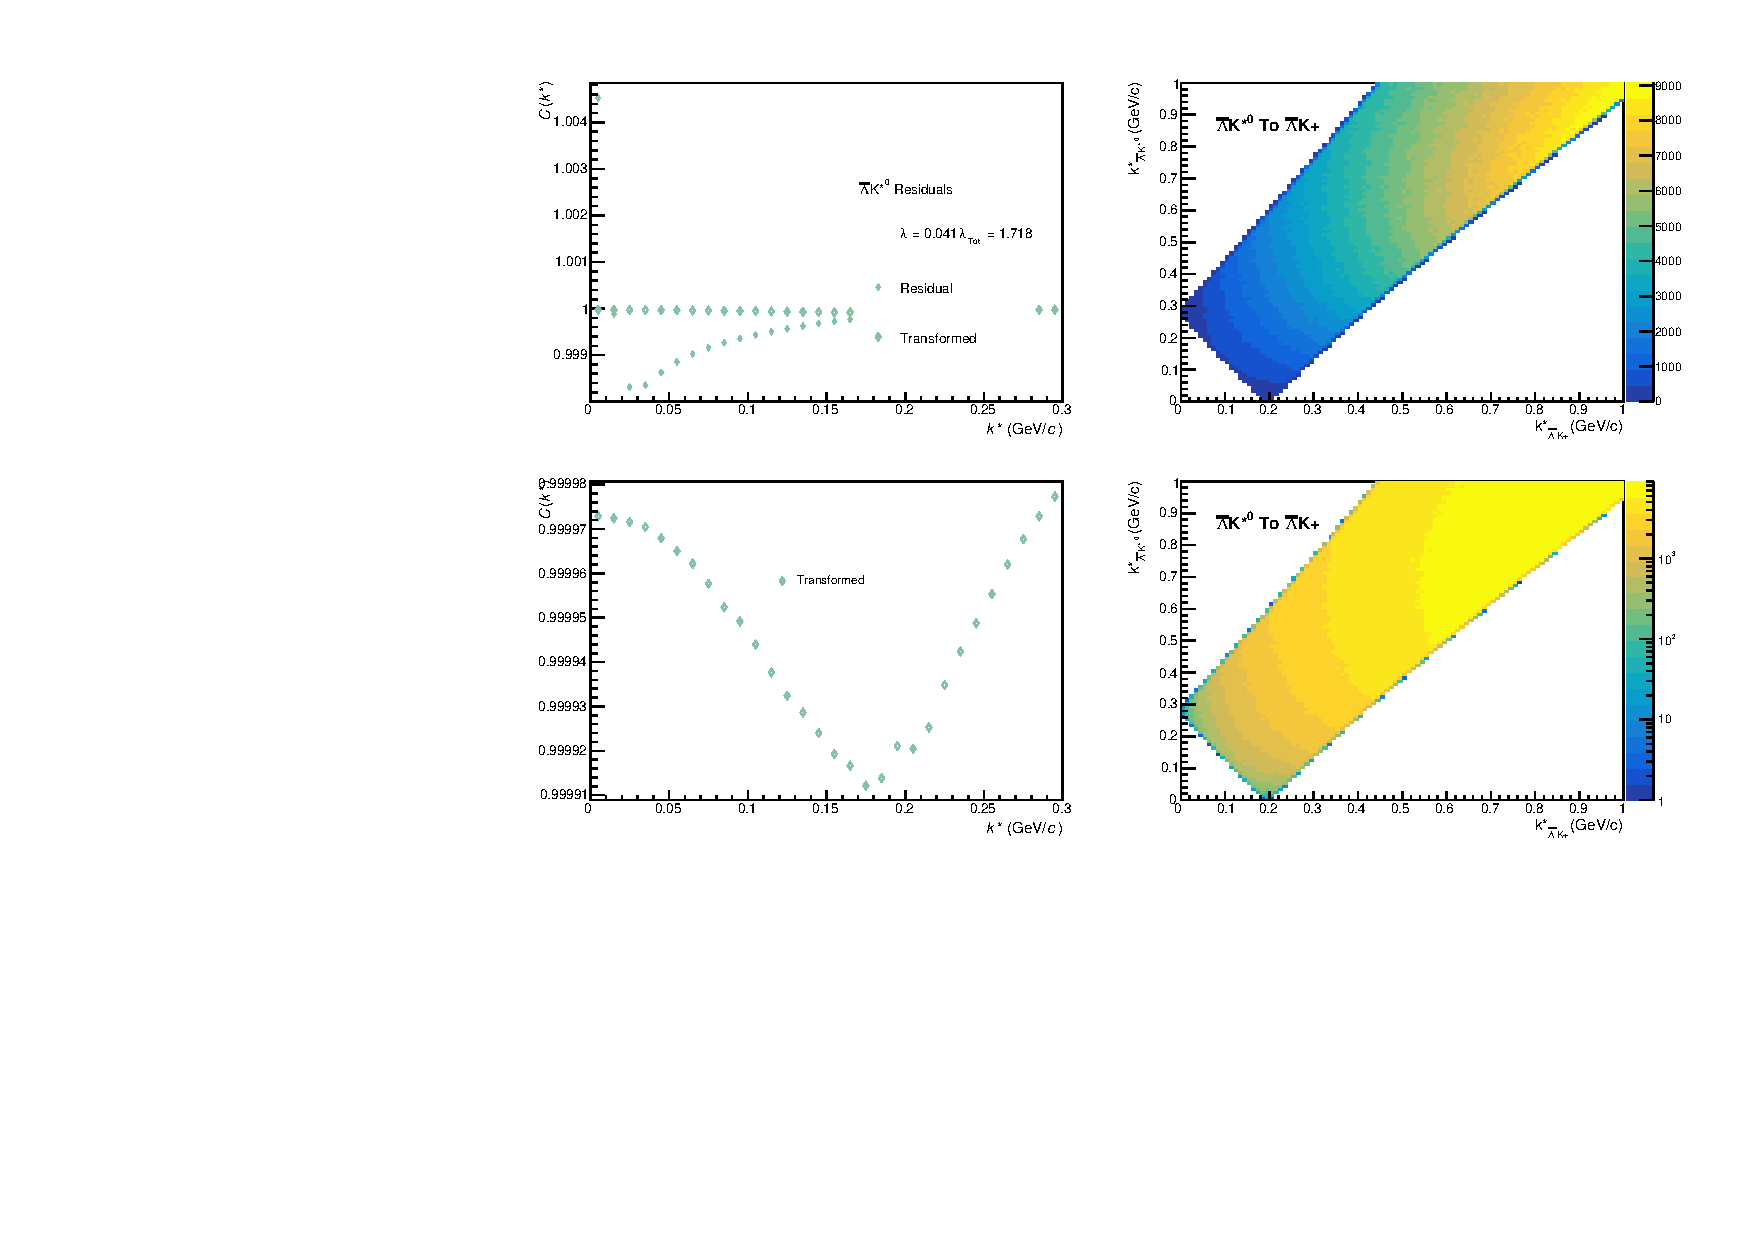
\includegraphics[width=\textwidth]{/home/jesse/Analysis/FemtoAnalysis/AnalysisNotes/Appendices/Appendix_AdditionalFigures/Figures/Residuals/ALamKchP/Residuals_ALamKchP_0010_ALamKSt0_MomResCrctn_NonFlatBgdCrctn_10Res_PrimMaxDecay4fm_UsingXiDataAndCoulombOnly.pdf}
  \caption[Residuals: $\bar{\Lambda}$K$^{*0}$ to $\bar{\Lambda}$K$^{+}$ (0-10\% Centrality)]{Residuals: $\bar{\Lambda}$K$^{*0}$ to $\bar{\Lambda}$K$^{+}$ (0-10\% Centrality)}
  \label{fig:Res_ALamKchP_0010_ALamKSt0}
\end{figure}


\begin{figure}[h]
  \centering
  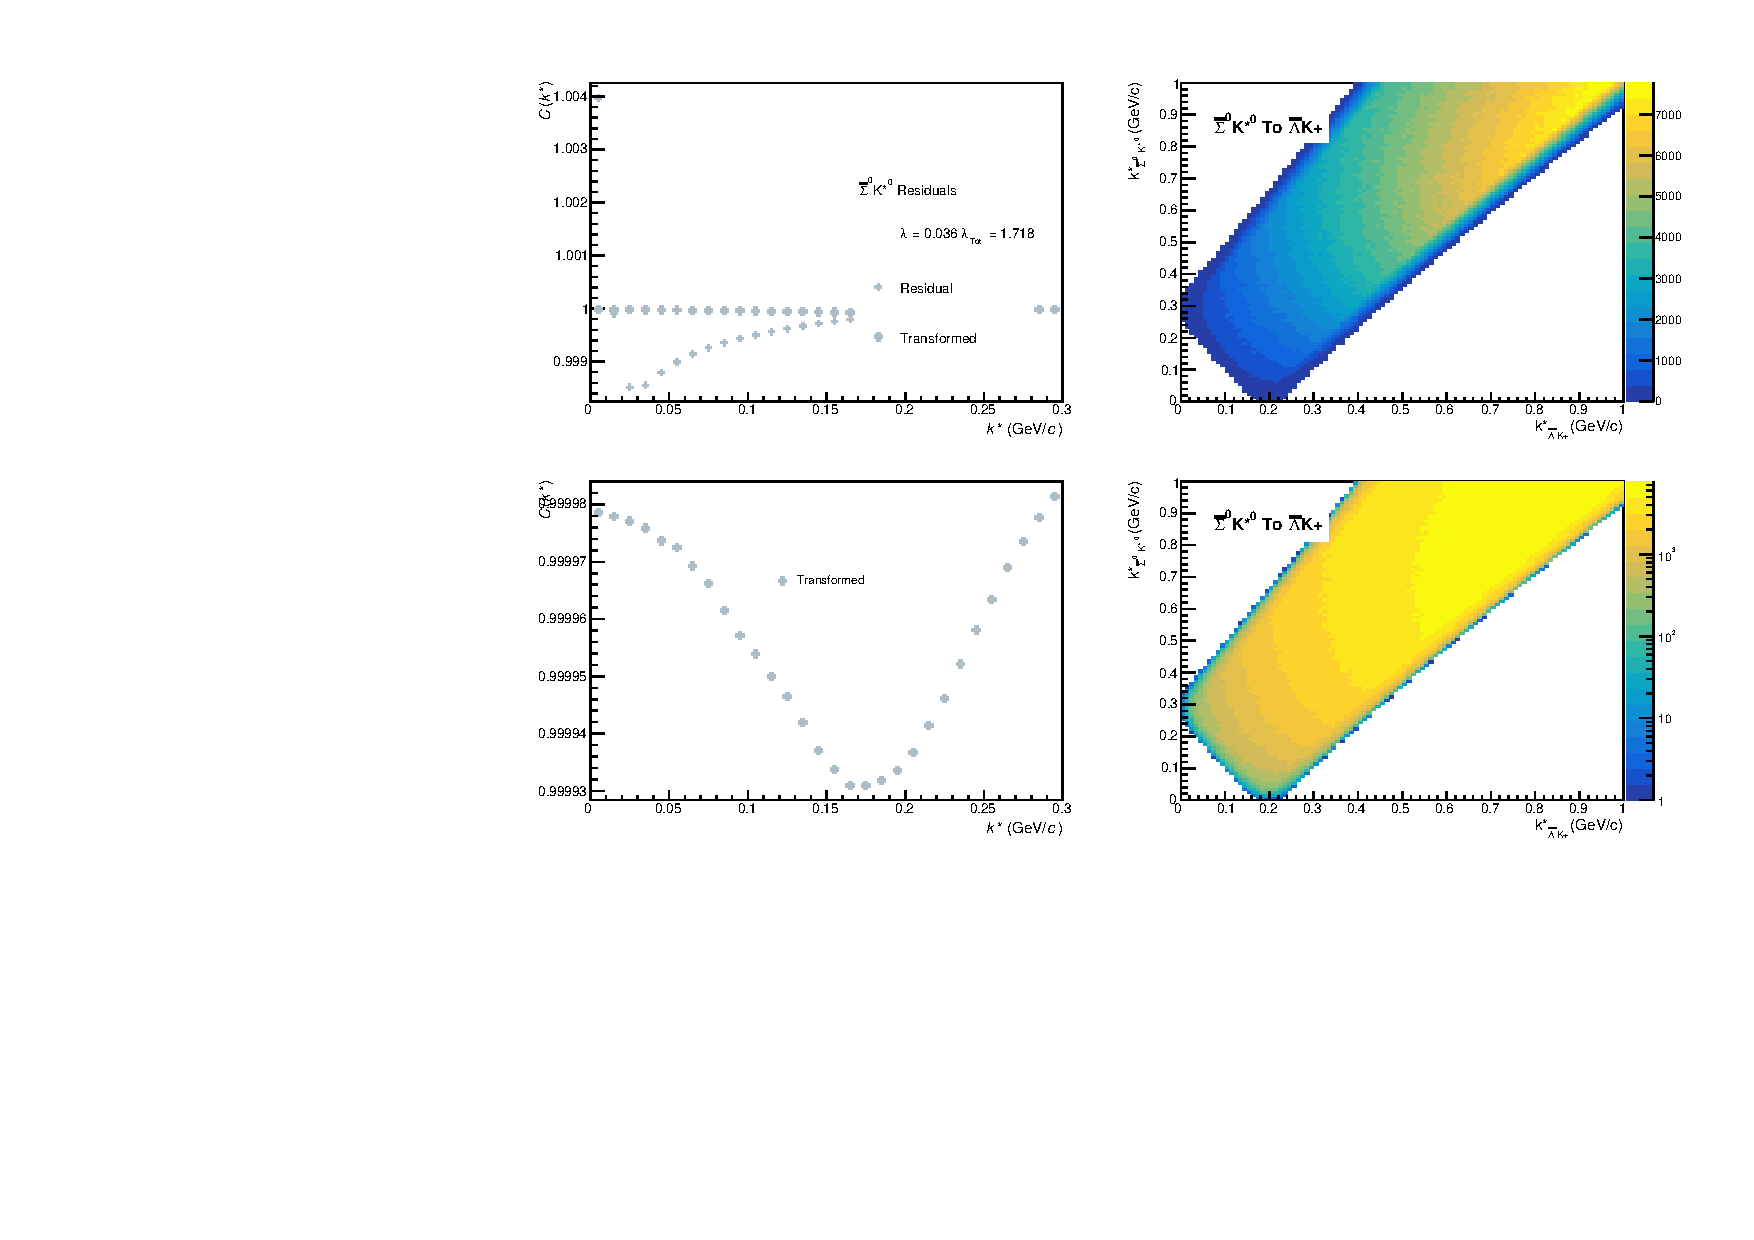
\includegraphics[width=\textwidth]{/home/jesse/Analysis/FemtoAnalysis/AnalysisNotes/Appendices/Appendix_AdditionalFigures/Figures/Residuals/ALamKchP/Residuals_ALamKchP_0010_ASig0KSt0_MomResCrctn_NonFlatBgdCrctn_10Res_PrimMaxDecay4fm_UsingXiDataAndCoulombOnly.pdf}
  \caption[Residuals: $\bar{\Sigma}^{0}$K$^{*0}$ to $\bar{\Lambda}$K$^{+}$ (0-10\% Centrality)]{Residuals: $\bar{\Sigma}^{0}$K$^{*0}$ to $\bar{\Lambda}$K$^{+}$ (0-10\% Centrality)}
  \label{fig:Res_ALamKchP_0010_ASig0KSt0}
\end{figure}


\begin{figure}[h]
  \centering
  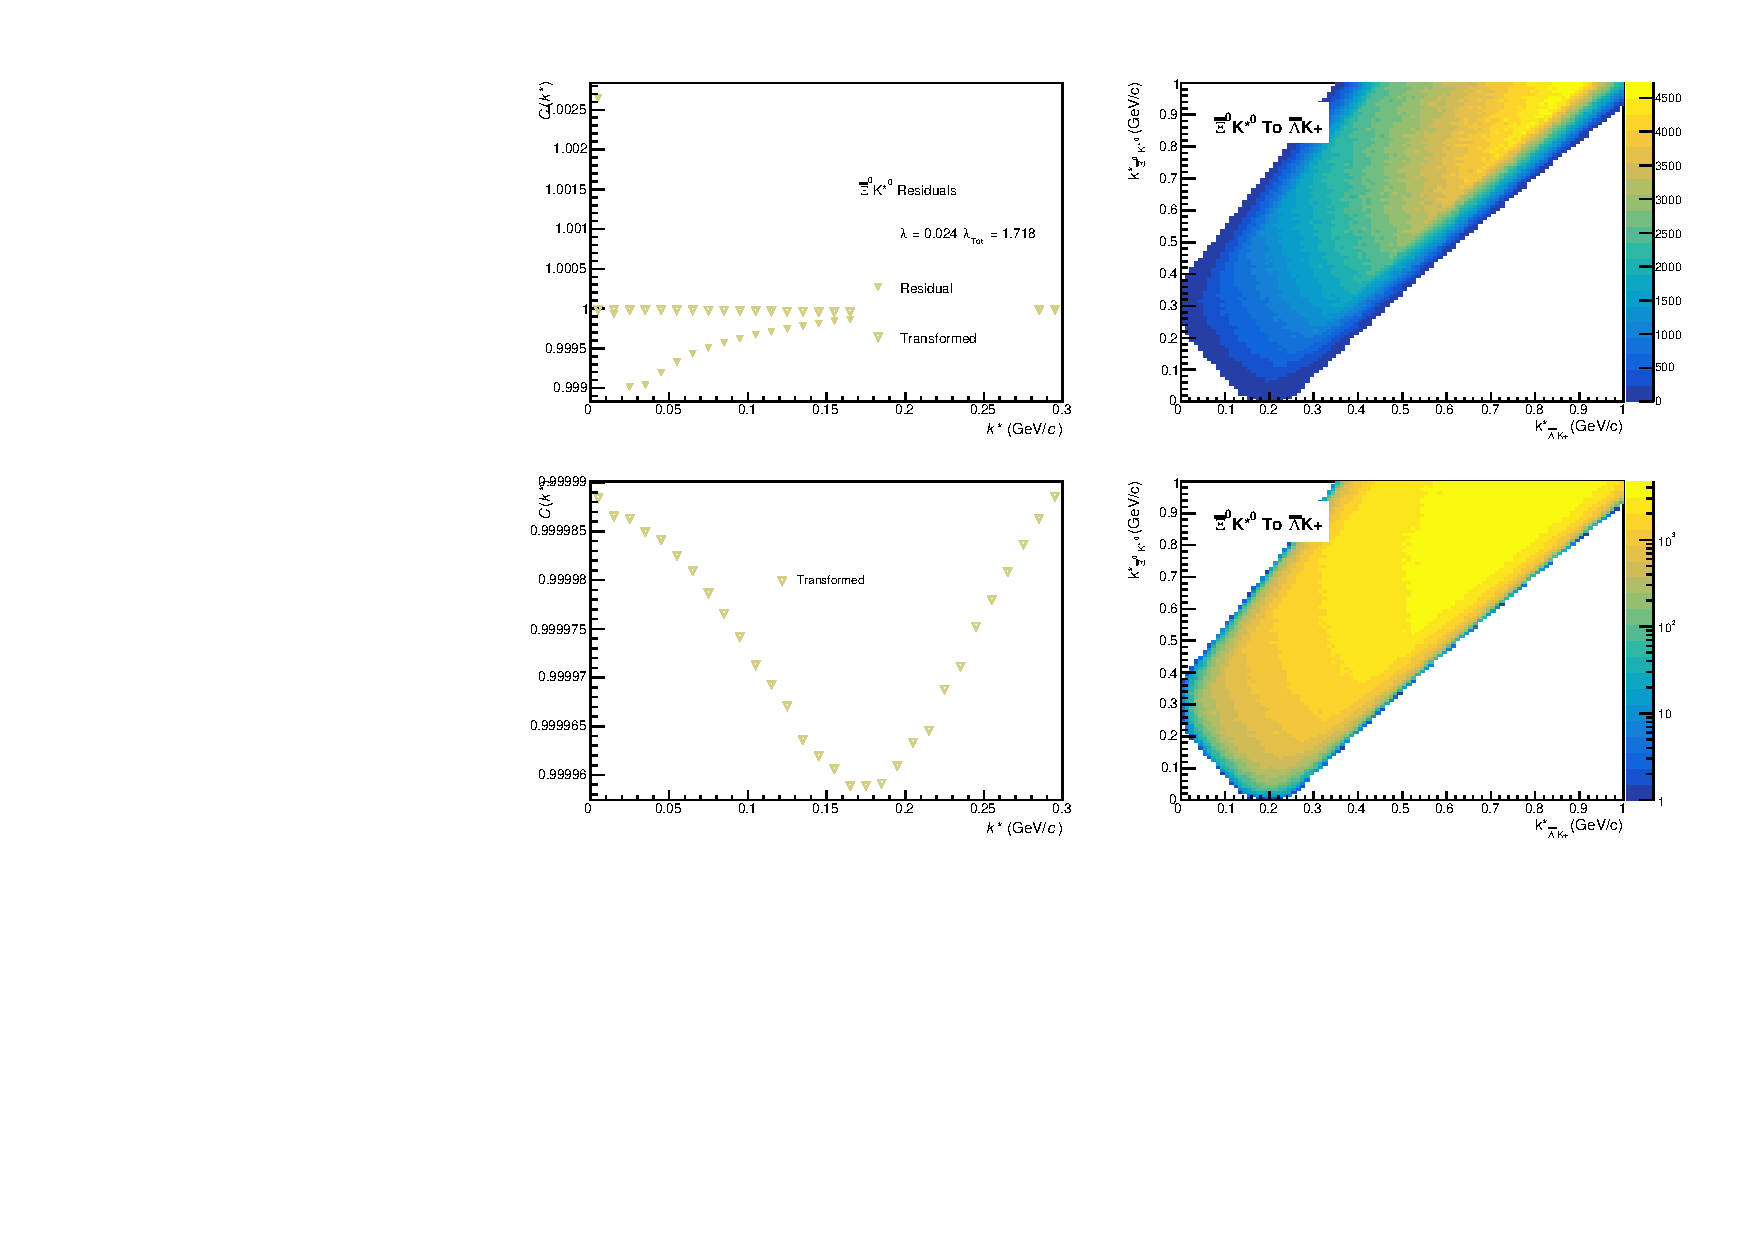
\includegraphics[width=\textwidth]{/home/jesse/Analysis/FemtoAnalysis/AnalysisNotes/Appendices/Appendix_AdditionalFigures/Figures/Residuals/ALamKchP/Residuals_ALamKchP_0010_AXi0KSt0_MomResCrctn_NonFlatBgdCrctn_10Res_PrimMaxDecay4fm_UsingXiDataAndCoulombOnly.pdf}
  \caption[Residuals: $\bar{\Xi}^{0}$K$^{*0}$ to $\bar{\Lambda}$K$^{+}$ (0-10\% Centrality)]{Residuals: $\bar{\Xi}^{0}$K$^{*0}$ to $\bar{\Lambda}$K$^{+}$ (0-10\% Centrality)}
  \label{fig:Res_ALamKchP_0010_AXi0KSt0}
\end{figure}

\begin{figure}[h]
  \centering
  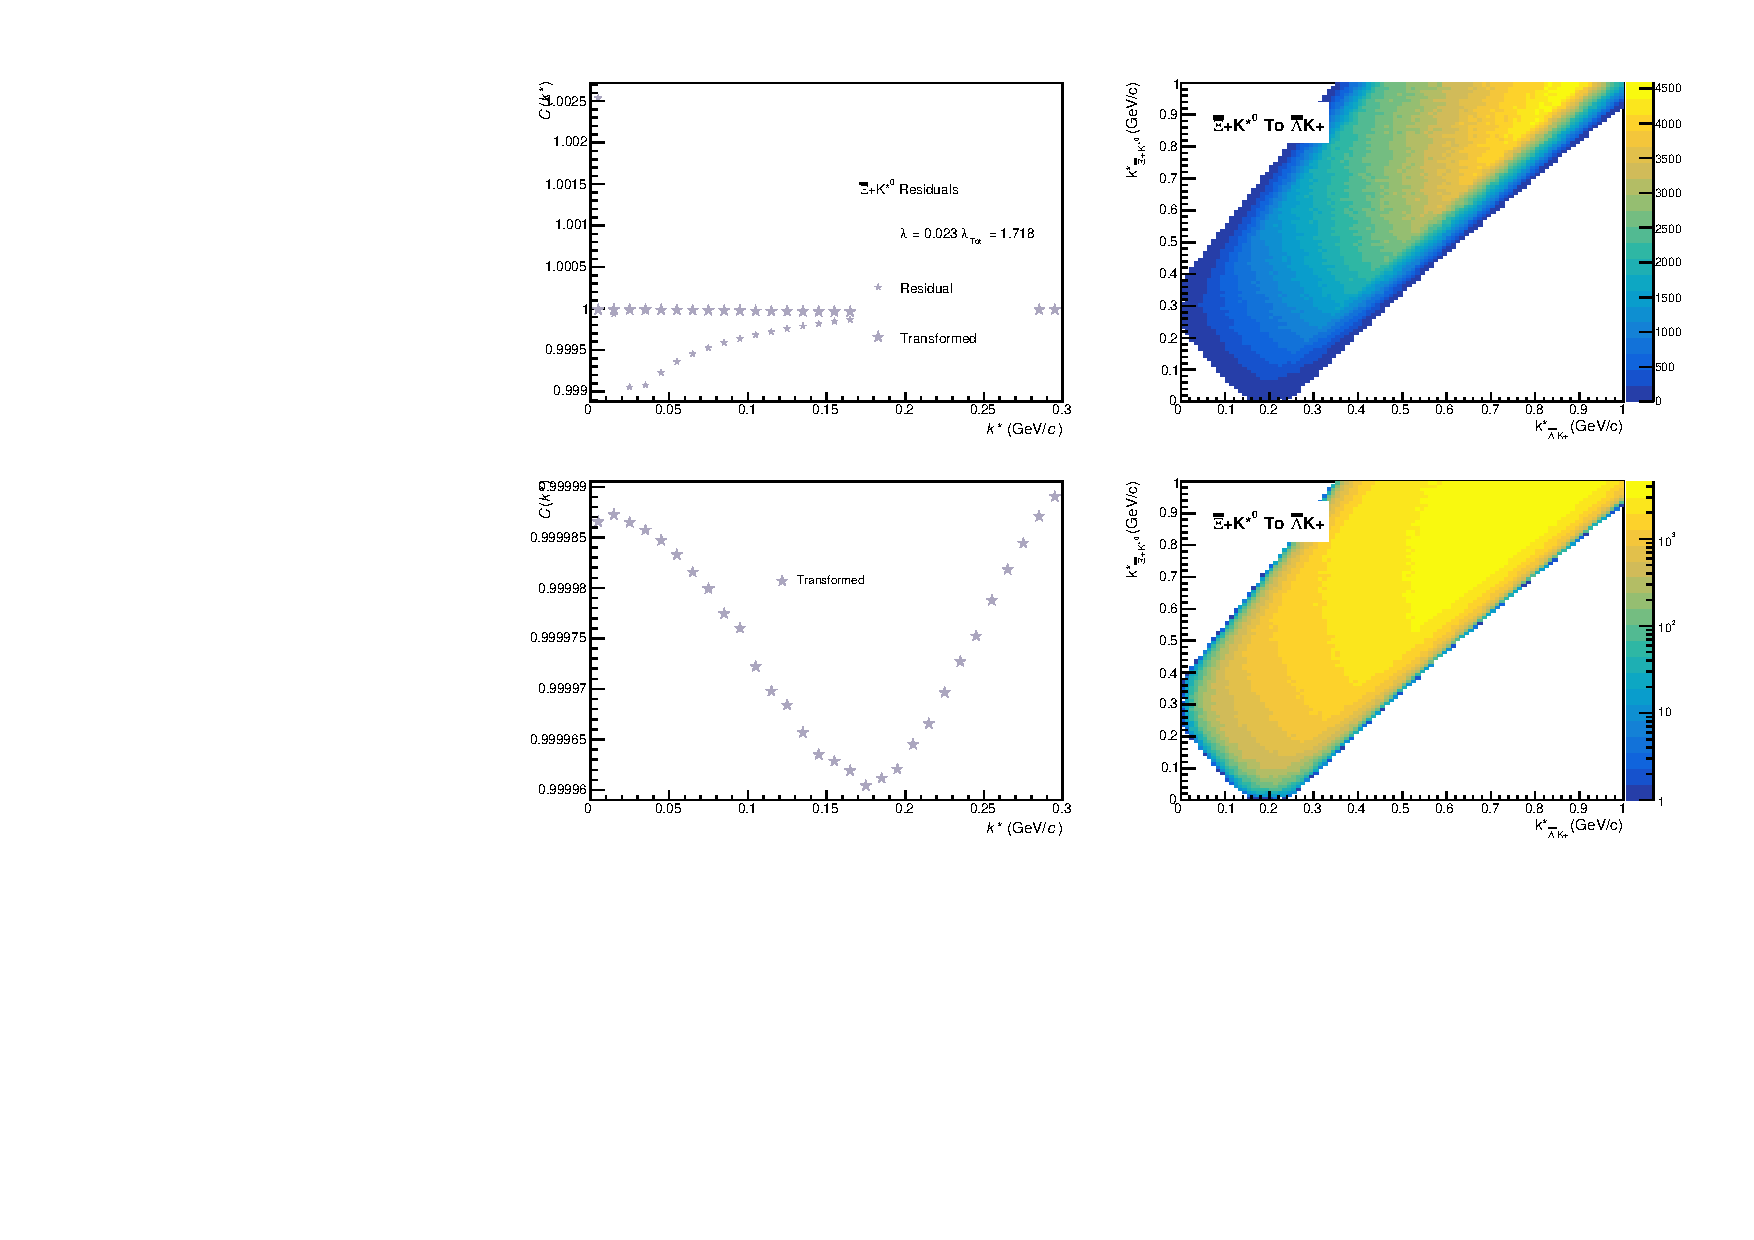
\includegraphics[width=\textwidth]{/home/jesse/Analysis/FemtoAnalysis/AnalysisNotes/Appendices/Appendix_AdditionalFigures/Figures/Residuals/ALamKchP/Residuals_ALamKchP_0010_AXiKSt0_MomResCrctn_NonFlatBgdCrctn_10Res_PrimMaxDecay4fm_UsingXiDataAndCoulombOnly.pdf}
  \caption[Residuals: $\bar{\Xi}^{+}$K$^{*0}$ to $\bar{\Lambda}$K$^{+}$ (0-10\% Centrality)]{Residuals: $\bar{\Xi}^{+}$K$^{*0}$ to $\bar{\Lambda}$K$^{+}$ (0-10\% Centrality)}
  \label{fig:Res_ALamKchP_0010_AXiCKSt0}
\end{figure}

\end{document}